\documentclass[a4paper,14pt,
%russcorr,
oneside]{extbook}
\usepackage[utf8]{inputenc}
\usepackage[T2A]{fontenc}
\usepackage[english,russian]{babel}
\usepackage{layout}
\usepackage{grfpaste}
\usepackage{floatflt}
\usepackage{datetime}
\usepackage{eso-pic,calc} %for background
\usepackage{graphicx}
\usepackage{corrcounters}
\usepackage[dvips]{geometry}
\usepackage{longtable} % для разбиения таблицы на несколько страниц
\usepackage{amssymb}
%\usepackage{cite} % for good citation 1-4
\usepackage{amsmath} %eqref command
 %\usepackage{epstopdf} % eps in miktex
\usepackage[toc,page]{appendix}
\usepackage{hhline}
\usepackage[shortlabels]{enumitem}
\usepackage{wrapfig}
\usepackage{comment}
\usepackage{float}
\usepackage{setspace}
\usepackage[pdfborder={0 0 0}]{hyperref}



\usepackage[style=gost-numeric, backend=biber, hyperref=auto, autolang=other, sorting=none, movenames=false]{biblatex}
\usepackage{csquotes}
\addbibresource{bib/my.bib}
\addbibresource{bib/my_conf.bib}

%\makeatletter
%\bibliographystyle{../ugost2008.bst}
%\renewcommand{\@biblabel}[1]{#1.}
%\providecommand*{\BibDash}{}
%\makeatother

\graphicspath{{fig/}, {../ch2_figures/}, {../ch3_figures/}, {../ch4_figures/},{../sign/}}

%\usepackage[unicode,colorlinks,citecolor=blue,linkcolor=blue,urlcolor=blue]{hyperref}

%%---- Оформление: разбиение текста на разделы и список литературы -----%%

\makeatletter   %% включение символа "@"

%--- изменение шрифтов и интервалов в секциях, подсекциях и главах ---%
\renewcommand{\section}{\@startsection{section}{1}
{0pt}{3.5ex plus 1ex minus .2ex} {2.3ex
plus.2ex}{\normalfont\large\bfseries}}
%{2.3ex plus.2ex}{\normalfont\normalsize\bfseries}}

\renewcommand{\subsection}{\@startsection{subsection}{2}
{0pt}{3.5ex plus 1ex minus .2ex} {2.3ex
plus.2ex}{\normalfont\normalsize\bfseries}}
%{2.3ex plus.2ex}{\normalfont\normalsize\slshape}}

\renewcommand{\@makeschapterhead}[1]{%
%\vspace*{0 pt}%
{\parindent=0pt \raggedright \normalfont\Large\bfseries #1\par
%\normalfont\normalsize\bfseries #1\par
\nopagebreak \vspace{5 pt}}}

%---------------------------------------------------------------------%

\renewcommand{\theequation}{\thesection.\arabic{equation}}   %% задали вид нумерации формул
\@addtoreset{equation}{section}

%\renewcommand{\@oddhead}{{\normalfont\slshape\rightmark}\hfill}   %% вид верхнего колонтитула
\renewcommand{\@oddhead}{}
\renewcommand{\@oddfoot}{\hfill \thepage \hfill}          %% вид нижнего колонтитула

\renewcommand{\@pnumwidth}{2em}   % увеличили пространство для номеров страниц в оглавлении

\makeatother   %% выключение символа "@"
%%----------------------------------------------------------------------%%


\voffset=-1in
\hoffset=-1in

\topmargin=0.8cm                 %% высота верхнего поля
\headheight=0.5cm
\headsep=0.7cm
\textheight=25.7cm %24.2cm       %% высота текста

\oddsidemargin=1.75cm %2cm        %% ширина левого поля
\textwidth=17.5cm                %% ширина текста

\addto\captionsrussian{
\def\figurename{Рис.}
\def\tabname{Таблица}
}

\renewcommand{\baselinestretch}{1.28}      %% межстрочный интервал

\renewcommand{\captionlinestretch}{1.28}   %% межстрочный интервал в подписях к рисункам
\renewcommand{\captionfontsize}{\normalsize}   %% размер шрифта в подписях к рисункам
\renewcommand{\captionwidth}{17.5cm}        %% ширина подписей к рисункам

%\newcommand{\scr}{\scriptstyle}
\newcommand{\ds}{\displaystyle}
%\newcommand{\ts}{\textstyle}

%\widowpenalty=10000\clubpenalty=10000   % запрет переноса первой/последней строки абзаца

\unitlength=1mm
%%-----------------------------------------------------------------------------%%

\renewcommand{\theequation}{\arabic{equation}}
\let\vaccent=\v % rename builtin command \v{} to \vaccent{}
\renewcommand{\v}[1]{\mathbf{#1}} % for vectors
\newcommand{\gv}[1]{\ensuremath{\mbox{\boldmath$ #1 $}}} 
% for vectors of Greek letters
\newcommand{\uv}[1]{\ensuremath{\mathbf{\hat{#1}}}} % for unit vector
\newcommand{\abs}[1]{\left| #1 \right|} % for absolute value
\newcommand{\avg}[1]{\left< #1 \right>} % for average
\let\underdot=\d % rename builtin command \d{} to \underdot{}
\renewcommand{\d}[2]{\frac{d #1}{d #2}} % for derivatives
\newcommand{\dd}[2]{\frac{d^2 #1}{d #2^2}} % for double derivatives
\newcommand{\pd}[2]{\frac{\partial #1}{\partial #2}} 
\newcommand{\pdone}[2]{\partial #1 / \partial #2} 
% for partial derivatives
\newcommand{\pdd}[2]{\frac{\partial^2 #1}{\partial #2^2}} 
% for double partial derivatives
\newcommand{\pdc}[3]{\left( \frac{\partial #1}{\partial #2}
 \right)_{#3}} % for thermodynamic partial derivatives
\newcommand{\ket}[1]{\left| #1 \right>} % for Dirac bras
\newcommand{\bra}[1]{\left< #1 \right|} % for Dirac kets
\newcommand{\braket}[2]{\left< #1 \vphantom{#2} \right|
 \left. #2 \vphantom{#1} \right>} % for Dirac brackets
\newcommand{\matrixel}[3]{\left< #1 \vphantom{#2#3} \right|
 #2 \left| #3 \vphantom{#1#2} \right>} % for Dirac matrix elements
\newcommand{\grad}[1]{\nabla #1} % for gradient
\let\divsymb=\div % rename builtin command \div to \divsymb
%\renewcommand{\div}[1]{\nabla \cdot #1} % for divergence
%\newcommand{\curl}[1]{\nabla \times #1} % for curl
\let\baraccent=\= % rename builtin command \= to \baraccent
\renewcommand{\=}[1]{\stackrel{#1}{=}} % for putting numbers above =
\renewcommand{\phi}{\varphi}
\def\No{\textnumero}

\def\v{\mathbf{v}}
\def\u{\mathbf{u}}
\def\x{\mathbf{x}}
\def\n{\mathbf{n}}
\def\V{\mathbf{V}}
\def\U{\mathbf{U}}
\def\F{\mathbf{F}}
\def\n{\mathbf{n}}
\def\c{\mathbf{c}}
\def\p{\mathbf{p}}
\def\d{\partial}
\def\om{\ensuremath{\mbox{\boldmath$\omega$}}} 
\def\Om{\ensuremath{\mbox{\boldmath$\Omega$}}} 
\def\rot{\mathop{}\!\operatorname{rot}}
\def\div{\mathop{}\!\operatorname{div}}
%\def\grad{\mathop{}\!\operatorname{grad}}
\def\grad{\nabla}
%\def\Laplace{\mathop{}\!\mathbin\bigtriangleup}
\def\Laplace{\mathop{}\!\Delta}
\def\Re{\operatorname{Re}}
%\def\i{\uv{i}}


\begin{document}

\righthyphenmin=2 \sloppy

\thispagestyle{empty}
\pdfbookmark[-1]{Численное исследование локализованных турбулентных структур в трубах}{title:link}
\centerline{МОСКОВСКИЙ ГОСУДАРСТВЕННЫЙ УНИВЕРСИТЕТ}
\centerline{имени M.В. ЛОМОНОСОВА}
%\centerline{МЕХАНИКО--МАТЕМАТИЧЕСКИЙ ФАКУЛЬТЕТ}

\vfill
 \rightline{\emph{На правах рукописи}}

\begin{figure}[h]
  \raggedleft
  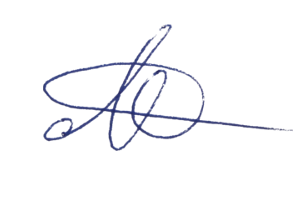
\includegraphics[height=2cm]{sign.png}
\end{figure}

\centerline{\bf Пиманов Владимир Олегович} \vfill
\centerline{\bf ЧИСЛЕННОЕ ИССЛЕДОВАНИЕ ЛОКАЛИЗОВАННЫХ}
\centerline{\bf ТУРБУЛЕНТНЫХ СТРУКТУР В ТРУБАХ}
 \centerline{\bf}
 \centerline{\bf }
\centerline{Специальность 01.02.05
--- Механика жидкости, газа и плазмы} 
\vfill \vfill
\centerline{АВТОРЕФЕРАТ}
\centerline{диссертации на соискание ученой степени} 
\centerline{кандидата физико--математических наук} 
\vfill \vfill \vfill \vfill 
\centerline{Mосква -- 2018}
\normalsize


\newcommand{\vsp}{\vspace{0.25cm}}

\newpage
\righthyphenmin=100
\thispagestyle{empty} Работа выполнена на кафедре гидромеханики механико-математического факультета МГУ имени М.В.~Ломоносова.
\righthyphenmin=2

\vsp

\noindent \begin{tabular}{@{}p{5.6cm}p{0.3cm}p{10.7cm}@{}}
Научный руководитель & -- & \textbf{Никитин Николай Васильевич},
доктор физико-математических наук, доцент\vsp \\
Официальные оппоненты &  -- & \textbf{Гайфуллин Александр Марксович},
доктор физико-математических наук, член-кор\-респондент РАН,
ФГУП <<Центральный аэрогидродинамический институт имени профессора Н.Е. Жуковского>>, главный научный сотрудник\vsp\\
&  & 
\textbf{Ильичёв Андрей Теймуразович},
доктор физико-математических наук, профессор,
ФГБУН <<Математический институт им. В.А. Стеклова РАН>>,
ведущий научный сотрудник\vsp\\
&  & 
\textbf{Ермаков Михаил Константинович},
кандидат физико-математических наук, ФГБУН <<Институт проблем механики им. А.Ю. Ишлинского РАН>>,
старший научный сотрудник\vsp\\
\end{tabular}
\vspace{1mm}

%\noindent 
Защита состоится 23 ноября 2018 г. в 15 часов на
заседании диссертационного совета МГУ.01.03 Московского
государственного университета имени М.В.~Ломоносова по адресу:
119991, ГСП--1, Москва, Ленинские горы, МГУ, д.~1, Главное здание, механико-математический
факультет, аудитория 16-10.

\vsp

E--mail: \href{pelevina.daria@gmail.com}{pelevina.daria@gmail.com}

\vsp

С диссертацией можно ознакомиться в отделе диссертаций научной библиотеки МГУ имени М.В.~Ломоносова (Ломоносовский просп., д.~27) и на сайте ИАС <<ИСТИНА>>: \url{https://istina.msu.ru/dissertations/146312517/}.

\vsp

Автореферат разослан <<\underline{\hspace{1.0cm}}>> октября 2018 г.

\vsp

\vfill

\noindent\begin{tabular}{@{}p{10cm}@{}p{4cm}@{}p{3.5cm}@{}}
Ученый секретарь

диссертационного совета,

кандидат физико-математических наук
 &
$\:$

$\:$

\vspace{-4mm}


\includegraphics[height=2cm]{psign.jpg}
 &
$\:$

$\:$

\raggedleft  Д.А. Пелевина\\
\end{tabular}

\newpage
\input description.tex
\input content.tex
\input conclusion.tex
\input publications.tex

\end{document}






